\addcontentsline{toc}{chapter}{SPRING}
\chapter*{SPRING}
\stepcounter{chapter}
\section{Spring Boot}
Es un framework similar a spring pero revivido. Lo esencial tiene 5 trucos que realiza:
\begin{enumerate}
\item \textbf{Configuración automática}
\end{enumerate}

\section{Spring inizializer}
Para comenzar con el proyecto de Spring Boot se deber ir a la página \url{https://start.spring.io/}, configurar y pulsar generar. 
\begin{figure}[h]
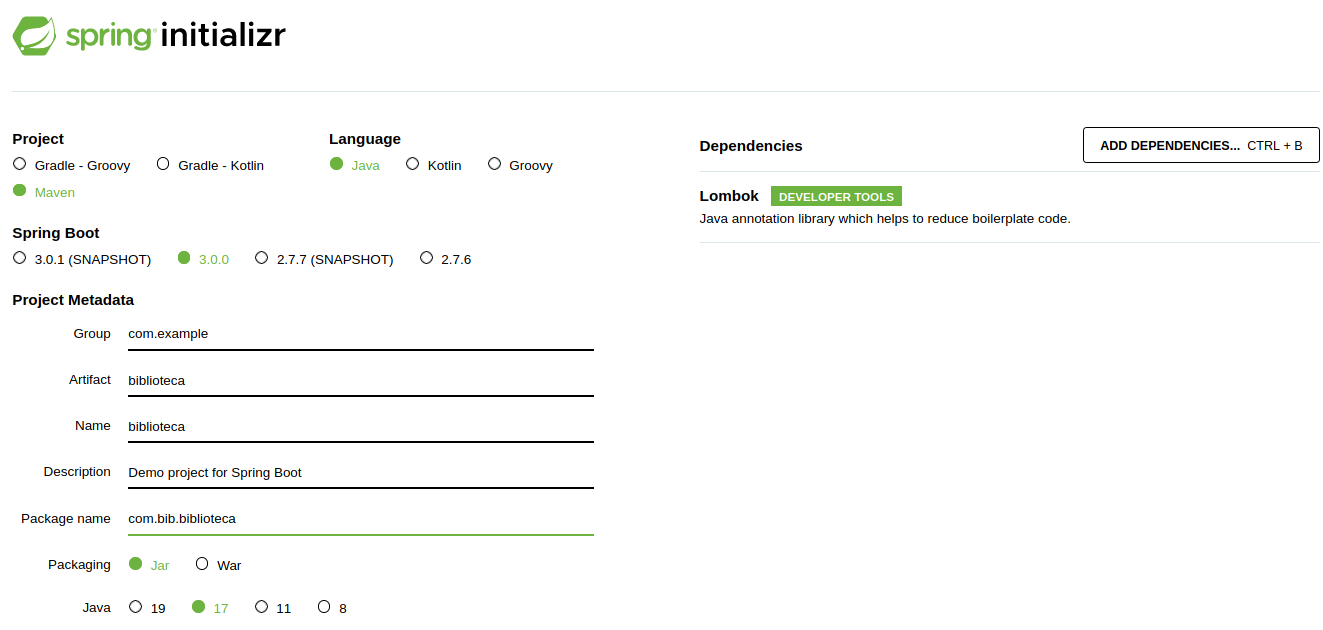
\includegraphics[scale=0.5]{images/spring1}
\caption{La configuración al iniciar un proyecto Spring Boot}
\end{figure}
Se verifica java para configurar. 
\begin{verbatim}
tomas@debian:~$ java --version
openjdk 17.0.4 2022-07-19
OpenJDK Runtime Environment (build 17.0.4+8-Debian-1deb11u1)
OpenJDK 64-Bit Server VM (build 17.0.4+8-Debian-1deb11u1, mixed mode, sharing)
\end{verbatim}


